\documentclass[11pt]{article}
\usepackage{graphicx,amsmath,amsfonts,hyperref}
\usepackage{natbib}
\usepackage[margin=1in]{geometry}
\hypersetup{colorlinks=true, linkcolor=blue, urlcolor=blue, citecolor=blue}

\title{Reproducing SDSS Spectral Compression Using a Standard Autoencoder}
\author{Zehao Peng}
\date{\today}

\begin{document}

\maketitle

\section{Introduction}
The Sloan Digital Sky Survey (SDSS) provides high-resolution optical spectra of galaxies that contain rich physical information, but the high dimensionality (typically 1000+ wavelength bins per spectrum) makes interpretation and visualization challenging. To address this, Portillo et al.\ \citep{Portillo2020} proposed using a Variational Autoencoder (VAE) to perform non-linear dimensionality reduction of galaxy spectra. In this project, I reproduce the core findings of their work using a standard (non-variational) autoencoder. This will be my CTA200 course project and is done as preparation for my research this summer. 

\section{Method}
\subsection{Data Processing}
The dataset contains $\sim$64,000 galaxy spectra from SDSS, originally compiled for the VAE study by Portillo et al. Each spectrum is sampled over 1000 wavelength bins ranging from approximately 3388 \AA{} to 8310 \AA{}. The raw spectra are reconstructed from PCA coefficients using the \texttt{sdss\_corrected\_spectra} utility from \texttt{astroML} \citep{VanderPlas2012}, then normalized by their respective PCA norms:
\begin{equation}
\mathbf{x}_i = \frac{\text{rawspec}_i}{\text{norm}_i},
\end{equation}
where $\mathbf{x}_i$ is the normalized spectrum of the $i$-th galaxy.

Normalization serves these main purposes: (1) it removes variations in total flux between galaxies, allowing the model to focus on spectral shape rather than brightness; (2) it stabilizes training by ensuring that all inputs have similar magnitudes; and (3) it aligns with the preprocessing used in the original VAE paper, enabling direct comparisons.

Each spectrum is associated with a pixel-wise error estimate $\sigma_i$, which is used to compute weights used later in the loss function:
\begin{equation}
\mathbf{w}_i = \frac{1}{\sigma_i^2 + \epsilon}, \quad \epsilon = \frac{1}{2 \times 10^6}
\end{equation}
$\epsilon$ is used to cap extremely small uncertainties and avoid exploding weights. Pixels with non-physical or flagged values (e.g., from bad sky subtraction) are masked using a boolean mask $\mathbf{m}_i$ and assigned zero weight:
\begin{equation}
\mathbf{w}_i[\mathbf{m}_i = 1] = 0.
\end{equation}

Please note that for a fair reproduction, all the data processing steps mirror exactly those from the work of Portillo et al. The dataset is randomly split into 47,000 training and 16,000 validation spectra. All data is converted to 32-bit floating point format for compatibility with Apple's MPS backend (my device). 

\subsection{Network Architecture and Training}
The autoencoder is a fully-connected feedforward neural network designed to compress and reconstruct the 1000-dimensional spectral input. It consists of two symmetric components:

\begin{itemize}
    \item \textbf{Encoder:} Maps the input spectrum $\mathbf{x} \in \mathbb{R}^{1000}$ to a latent representation $\mathbf{z} \in \mathbb{R}^6$ via:
    \begin{align*}
        \mathbf{h}_1 &= \text{ReLU}(\mathbf{W}_1 \mathbf{x} + \mathbf{b}_1), \quad \mathbf{W}_1 \in \mathbb{R}^{703 \times 1000} \\
        \mathbf{h}_2 &= \text{ReLU}(\mathbf{W}_2 \mathbf{h}_1 + \mathbf{b}_2), \quad \mathbf{W}_2 \in \mathbb{R}^{94 \times 703} \\
        \mathbf{z} &= \mathbf{W}_3 \mathbf{h}_2 + \mathbf{b}_3, \quad \mathbf{W}_3 \in \mathbb{R}^{6 \times 94}
    \end{align*}

    \item \textbf{Decoder:} Reconstructs $\hat{\mathbf{x}}$ from the latent representation:
    \begin{align*}
        \mathbf{h}_3 &= \text{ReLU}(\mathbf{W}_4 \mathbf{z} + \mathbf{b}_4), \quad \mathbf{W}_4 \in \mathbb{R}^{94 \times 6} \\
        \mathbf{h}_4 &= \text{ReLU}(\mathbf{W}_5 \mathbf{h}_3 + \mathbf{b}_5), \quad \mathbf{W}_5 \in \mathbb{R}^{703 \times 94} \\
        \hat{\mathbf{x}} &= \mathbf{W}_6 \mathbf{h}_4 + \mathbf{b}_6, \quad \mathbf{W}_6 \in \mathbb{R}^{1000 \times 703}
    \end{align*}
\end{itemize}

The autoencoder is trained by optimizing the trainable parameters $\theta$, which include all weights and biases in the encoder and decoder networks. The objective is to minimize a weighted mean squared error (MSE) loss over the training data:
\begin{equation}
\theta^* = \arg\min_\theta \mathcal{L}(\mathbf{x}, \hat{\mathbf{x}}_\theta, \mathbf{w}) = \frac{1}{N} \sum_{i=1}^{N} \sum_{j=1}^{1000} w_{ij} (x_{ij} - \hat{x}_{ij})^2
\end{equation}
where $\hat{\mathbf{x}}_\theta$ is the network’s reconstruction of $\mathbf{x}$ given parameters $\theta$, $N$ is the batch size, and $j$ indexes the wavelength bins. This formulation is an inverse-variance-weighted MSE, where each pixel's contribution to the loss is scaled by the reciprocal of its squared uncertainty. This emphasizes high signal-to-noise regions of the spectrum while appropriately down-weighting noisier or masked pixels. This is analogous to the loss function used by Portillo et al. The network hyperparameters are chosen per Portillo et al.'s findings, which show that 6 latent parameters and a 1000-703-94-6-94-703-1000 architecture achieve the best results in terms of reconstruction loss. This setup is the point beyond which further increases in model capacity yielded diminishing improvements. The intuition behind this autoencoder is that by setting minimizing reconstruction loss as the optimization objective and forcing the model to funnel information through a `bottleneck', the latent parameters will capture the features most important for a high-fidelity reconstruction. In essence, this is similar to PCA. However, we are not restricted to reconstructing the spectra only via linear combinations of the latent parameters, which can yield a more interesting feature map. (Latent space)

Training was conducted using PyTorch Lightning \citep{Falcon2019}, which simplifies training loop management, and tracked using Weights \& Biases \citep{Biewald2020}. Training is performed using the Adam optimizer \citep{adam} with an initial learning rate of $10^{-3}$. Essentially, we are performing a variation of stochastic gradient descent on the loss landscape, with the goal of reaching a global minimum. The learning rate corresponds to the step size of this descent. A \texttt{ReduceLROnPlateau} scheduler reduces the learning rate by a factor of 10 after 5 epochs of no improvement in validation loss. Early stopping halts training if no improvement is seen for 10 consecutive epochs. This training regimen is also taken from Portillo et al.

Figure~\ref{fig:architecture} shows the architecture schematic of the model.

\begin{figure}[h!]
    \centering
    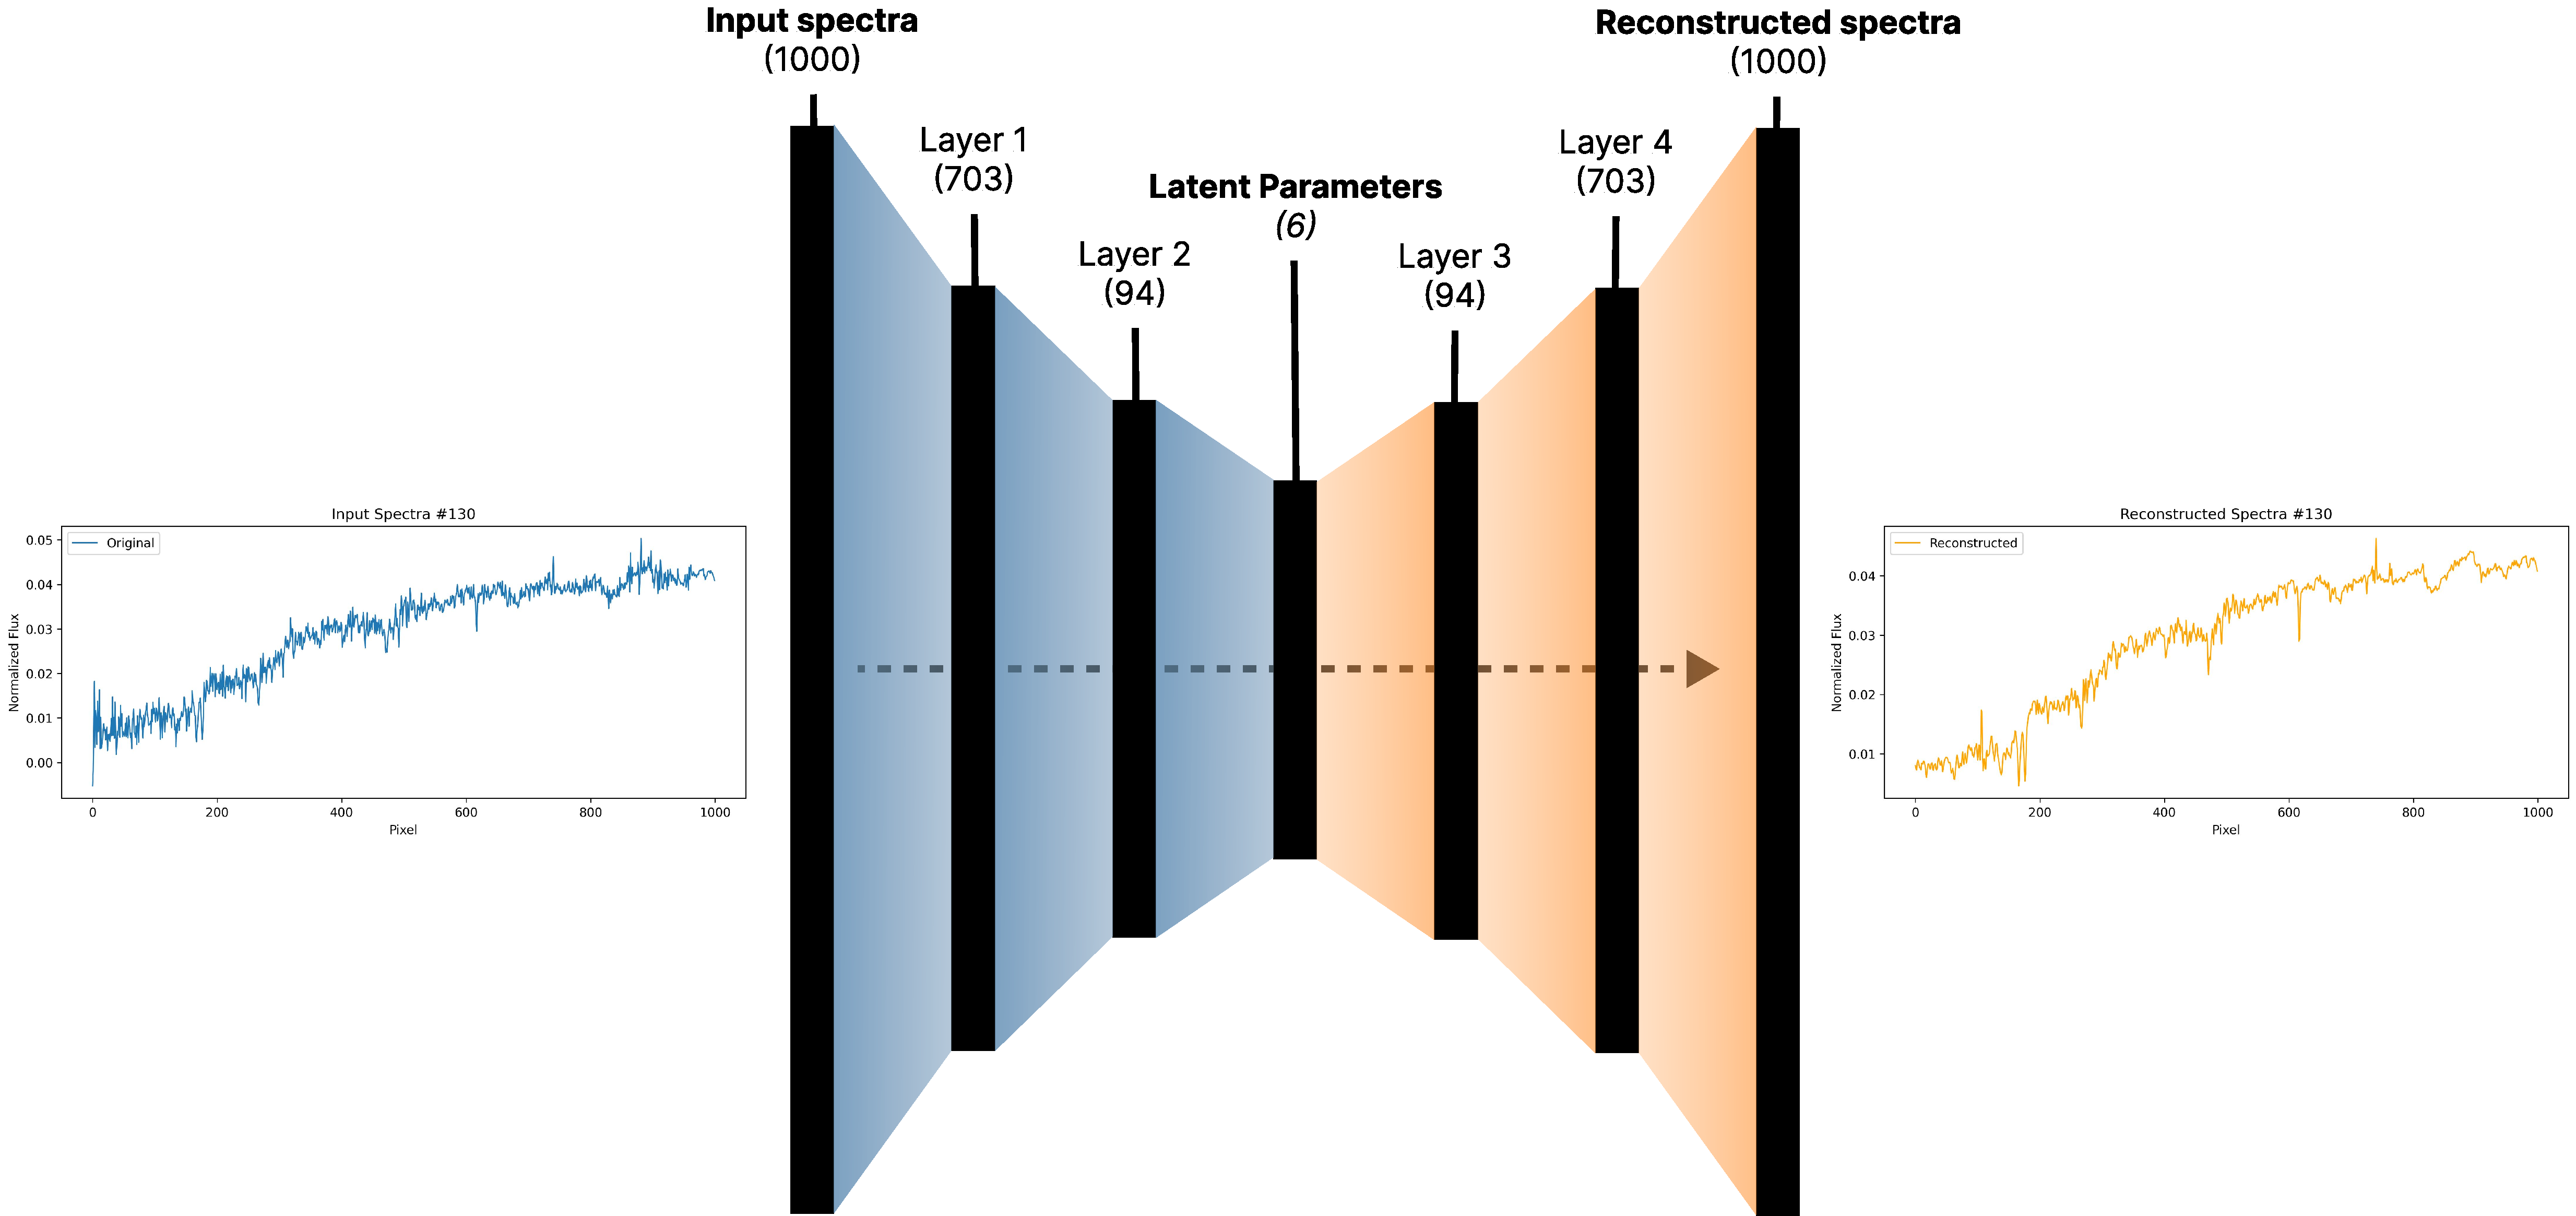
\includegraphics[width=\textwidth]{autoencoder_schematic.pdf}
    \caption{Schematic diagram of the autoencoder architecture used in this project.}
    \label{fig:architecture}
\end{figure}

\section{Results}
\subsection{Latent Space Representation}
After training until validation loss convergence, the 6-dimensional latent representations are visualized using corner plots and UMAP projections. These show clustering by galaxy spectral type, similar to the results of Portillo et al.

Figure~\ref{fig:cornerplot} illustrates the distribution of the latent parameters.

\begin{figure}[h!]
    \centering
    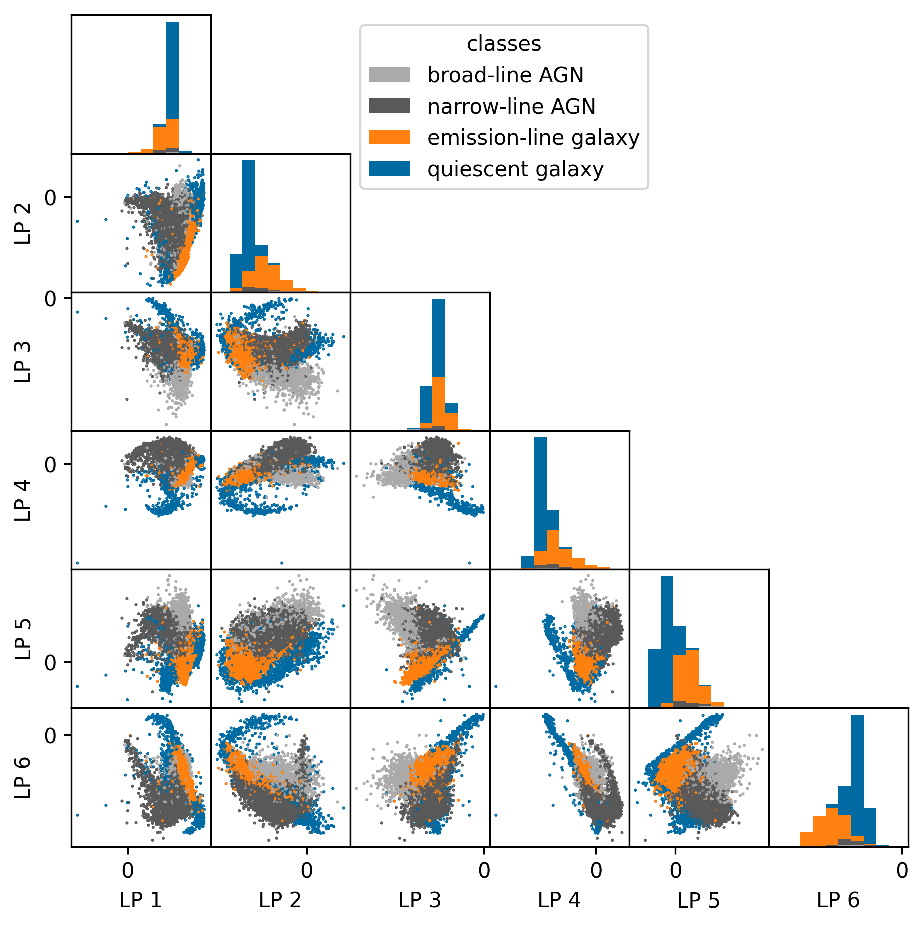
\includegraphics[width=0.9\textwidth]{corner.pdf}
    \caption{Corner plot showing the distribution of the 6 latent parameters across the dataset.}
    \label{fig:cornerplot}
\end{figure}

The clustering of spectra by galaxy type indicates that the learned latent parameters can differentiate between physically distinct spectral classes for quiescent, emission line, narrow-line AGN, and broad-line AGN galaxies, suggesting that the autoencoder successfully captures key features of galaxy spectra in its low-dimensional representation.

We may also see this clustering behaviour more clearly by further compressing the six latent parameters into two via means of the Uniform Manifold Approximation Program (UMAP), which again applies a non-linear dimensionality reduction to our latent space.

Figure~\ref{fig:umap} shows the result.

\begin{figure}[h!]
    \centering
    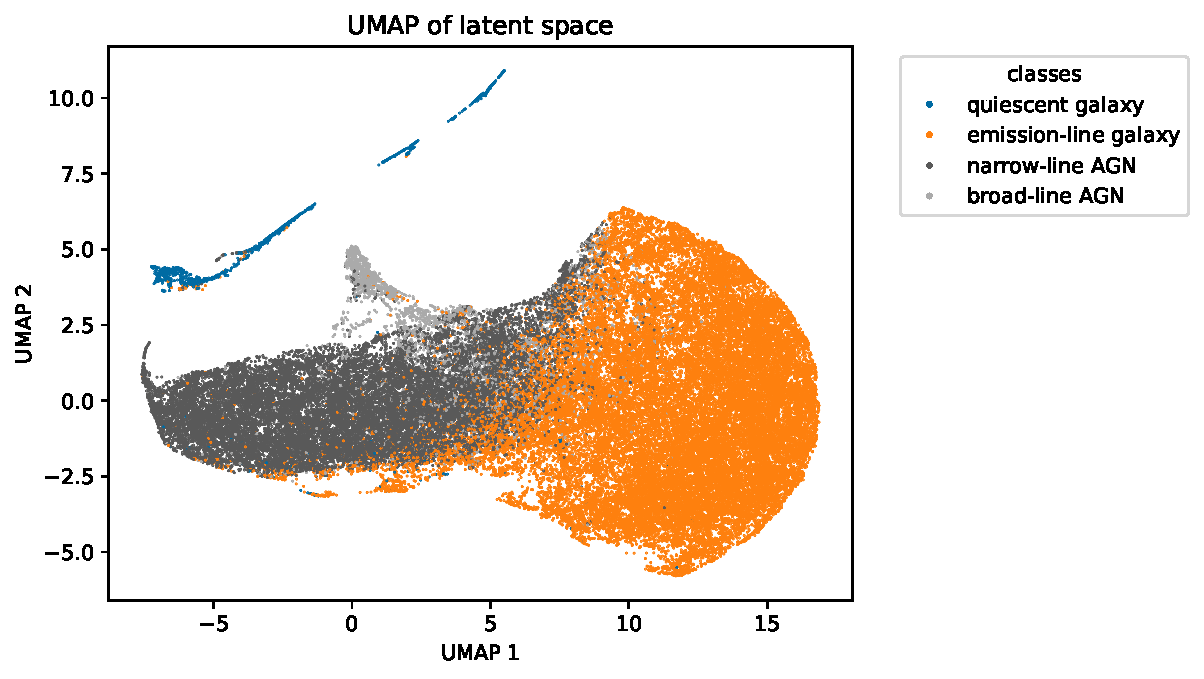
\includegraphics[width=\textwidth]{umap.pdf}
    \caption{2D UMAP embedding of the 6D latent space.}
    \label{fig:umap}
\end{figure}

Observe that the UMAP space has been roughly partitioned into four distinct regions corresponding to quiescent, emission line, narrow-line AGN, and broad-line AGN galaxies, coloured accordingly. This separation again indicates that the latent parameters are good discriminators of galaxy type. Due to the nature of UMAP, these axes are not very meaningful. They are therefore simply named UMAP1 and UMAP2.

\subsection{Spectral Reconstruction}
We will now examine its performance in spectral reconstruction.

Figure~\ref{fig:spectra} shows one such example.

\begin{figure}[h!]
    \centering
    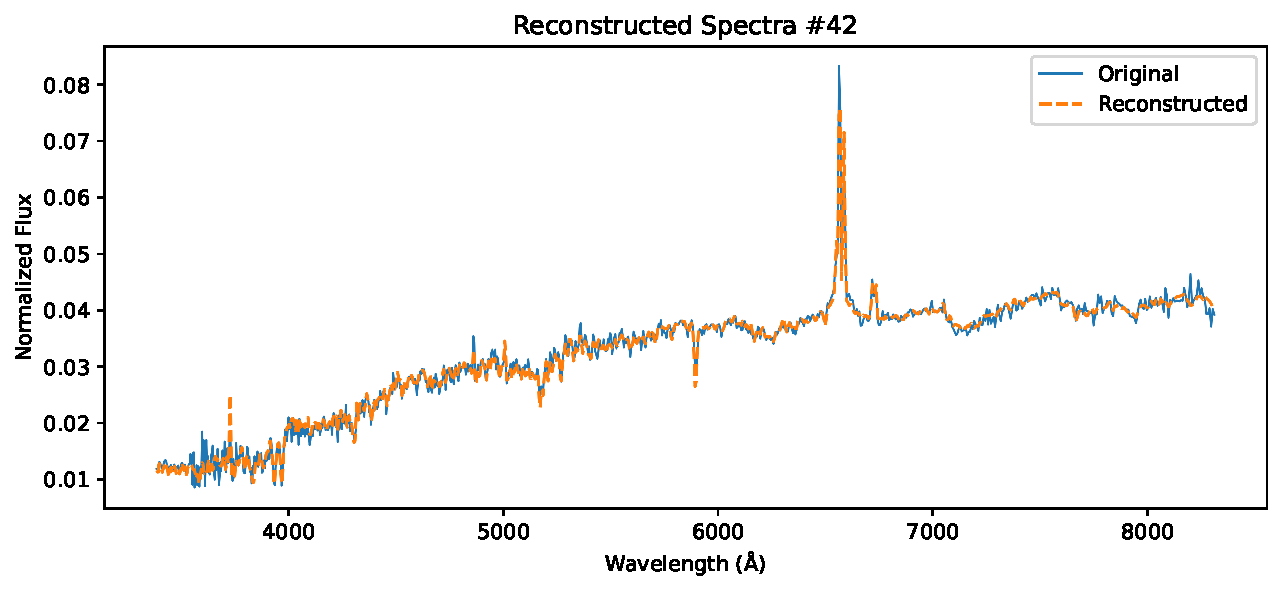
\includegraphics[width=0.9\textwidth]{spectrum_recon.pdf}
    \caption{Randomly selected example of reconstructed spectra (orange) compared to original input spectra (blue).}
    \label{fig:spectra}
\end{figure}

Notice that the general shape is captured very well, and the emission line around 6500 \AA{} (possibly the $H\alpha$ line) is reconstructed correctly.

To further evaluate reconstruction quality, we generate a 2D histogram of residuals (difference between input and reconstruction). This visualization helps assess whether reconstruction errors are systematically correlated with spectral features or uncertainty levels.

Figure~\ref{fig:residual_histogram} displays this.

\begin{figure}[h!]
    \centering
    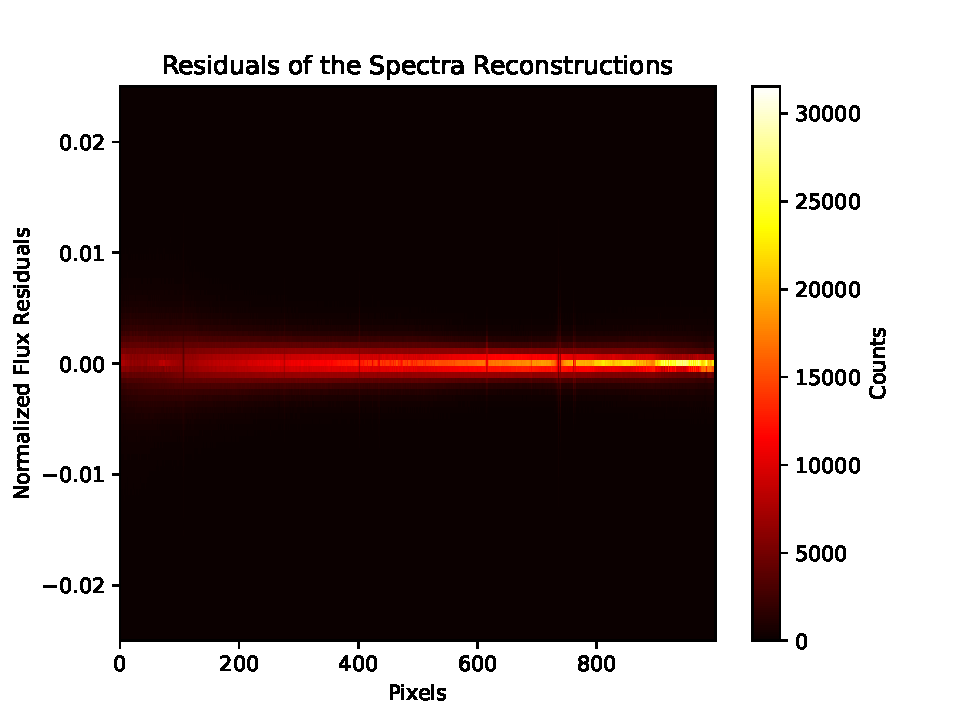
\includegraphics[width=0.9\textwidth]{residuals.pdf}
    \caption{2D histogram of reconstruction residuals binned by wavelength and residual flux.}
    \label{fig:residual_histogram}
\end{figure}

Notice that in general, residuals are tightly distributed around 0, with flux deviations usually no more than 0.05 in either direction. This indicates that the reconstructions are generally very accurate. We also notice, however, that there are vertical bands at common emission line wavelengths (e.g., $H\alpha$, [OIII], [NII]), which indicate that the autoencoder struggles to fully reconstruct narrow, high-contrast features. We see a specific example of this in Figure 4, where the reconstruction underpredicts the narrow but significant emission line.

\section{Conclusion}
This project demonstrates that a standard autoencoder can reproduce many of the core results of Portillo et al. (2020), including accurate spectrum reconstructions and, consequentially, a meaningful latent space capable of separating galaxies based on their spectrum. 

\bibliographystyle{aasjournal}
\bibliography{references}

\end{document}